\documentclass[a4paper, 12pt]{article}

\usepackage[left = 3cm, top = 3cm, bottom = 3cm, right = 2cm]{geometry}
\usepackage{graphicx}
\usepackage[spanish,es-tabla]{babel} % Idioma español con tablas
\usepackage{amsmath}
\usepackage{amssymb}
\usepackage{amsfonts}
\usepackage[utf8]{inputenc}         % Para escribir en castellano
\usepackage[T1]{fontenc}
\usepackage{color}
\usepackage{alltt}
\usepackage{times}
\usepackage{setspace}  % Usado para doble espacio, espacio y medio y espacio simple
\usepackage{booktabs}         % Para formar tablas
%\usepackage{longtable}       % Usado para diseñar grandes tablas.
%\usepackage[round]{natbib} 
\usepackage[numbers]{natbib}
\usepackage{url}
\urlstyle{same}
\bibliographystyle{ieeetr}

\usepackage[x11names,table]{xcolor}

\begin{document}

\begin{center}
 {\bf {\fontsize{16}{16.8}\selectfont UNIVERSIDAD NACIONAL DE TRUJILLO}}     
 \vskip 0.15cm
    {\bf{\fontsize{16}{16.8}\selectfont Facultad de Ciencias Físicas y Matemáticas}} 
\vskip 0.15cm
  {\bf{\fontsize{16}{16.8}\selectfont Escuela Profesional de Informática}}
\end{center}  

\begin{figure}[ht]
\begin{center}

\includegraphics[width=.3\textwidth]{unt}
\end{center}
\end{figure}

\vskip 2cm

\begin{center}
  { \bf {\fontsize{17}{20.4} \selectfont{ Desarrollo de un sistema BMS – IoT y su influencia en el \\ 
  \vskip 0.2cm control automatizado del consumo eléctrico basado en el\\
  \vskip 0.2cm protocolo MQTT en viviendas multifamiliares,\\
  \vskip 0.2cm Trujillo 2023.}}  } 
%\end{center}  

 
  \vskip 2cm
  { \bf {\fontsize{17}{20.4}\selectfont{\hspace*{-0.4cm}Autores: }}  }
  
 \vskip 0.25cm 
  
   Daniel Iván Cruz Flores \\
   Leoncio Marubi Moya Carranza
 
	   
  \vskip 1cm
  { \bf {\fontsize{17}{20.4}\selectfont{\hspace*{-0.4cm}Asesor: } }  } 
 \vskip 0.25cm 
 
   Dra. Patricia Pereyra Salvador
  
\vskip 2cm


%\begin{center}    
{\bf {\fontsize{14}{16.8}\selectfont Trujillo - La Libertad
\vskip 0.0cm
\hspace*{-0.2cm} 
\vskip 0.1cm
2023 }}
\end{center} 
\newpage

\begin{center}
%\onehalfspace  \doublespacing  \singlespace
\Large {PROYECTO DE INVESTIGACIÓN DE TESIS \\
\vskip 0.2cm
 ESCUELA PROFESIONAL DE INFORMÁTICA}
\end{center}
\vskip 1cm

\section{GENERALIDADES}
%De acuerdo con  \cite{Erica} las investigaciones nacen de una idea, sin importar qué tipo de paradigma fundamente el estudio ni el enfoque que se habrá de seguir. Para dar inicio a la investigación se necesita primero, la idea que éste será el primer acercamiento a lo que realmente se quiere investigar o al ambiente al cual  habra que estudiar. \par
%\vskip 0.3cm
%La investigación es la realización de un trabajo de búsqueda, mediante el uso del método científico, para adquirir conocimientos científicos y describir, explicar y predecir los fenómenos que ocurren en esa pequeña parte de universo que se quiere estudiar y conocer.               



\subsection{Título}
Desarrollo de un sistema BMS – IoT y su influencia en el control automatizado del consumo eléctrico basado en el protocolo MQTT en viviendas multifamiliares, Trujillo 2023.

\subsection{Autor(es)}
%Indicar apellidos y nombres de los participantes:
\begin{table}[h!]
 \caption{\small{Datos de los investigadores}}
\begin{tabular}{llrrr} \toprule
{\bf Código(s)} & {\bf Nombres y Apellidos} & {\bf Cargo en el proyecto} & {\bf Email} \\ \midrule
512701004 & Daniel I. Cruz Flores & investigador  & ivan17cf@gmail.com \\
022700305    & Leoncio M. Moya Carranza & investigador  & leonciomoya@gmail.com            \\ \bottomrule
\end{tabular}
\end{table}



\subsection{Tipo de investigación}

\begin{itemize}
\item De acuerdo al fin que se persigue: Aplicada 
\item De acuerdo al alcance de  la investigación: Descriptiva experimental.
\end{itemize}



\subsection{Áreas de Investigación}
\begin{itemize}
\item Redes y comunicación.
\item Lenguajes de programación.
\item Ingeniería de software.
\item Sistemas operativos.
\item Desarrollo basado en plataforma.
\end{itemize}
\subsection{Líneas de Investigación}
\begin{itemize}
\item Entrega de datos confiable.
\item Programación orientada a objetos.
\item Construcción de software.
\item Sistemas de tiempo real embebidos.
\item Plataforma web.

\end{itemize}

               
\subsubsection{Tema de investigación :} 

El protocolo de red MQTT y su aplicación en soluciones IoT

\subsection{Localidad e Institución donde se desarrollará el proyecto }

\begin{itemize}

\item Localidad: 
Departamento de la Libertad, Provincia de Trujillo, distrito de Trujillo.

\item Institución: 
Universidad Nacional de Trujillo / Facultad de ciencias físicas y matemáticas/ Informática.

\end{itemize}

\subsection{Duración del trabajo de tesis (Plan y desarrollo)}
%Ejemplo:\\
\hspace*{0.7cm}Del \hspace*{0.2cm}27/02/2023 \hspace*{0.3cm} AL\hspace*{0.2cm}27/05/2023  \hspace*{0.2cm}(03 meses)
 
\subsection{Cronograma del trabajo de investigación y desarrollo}
%\subsubsection{Cronograma del plan TG y avance del desarrollo TG (un ciclo) }

 \begin{table}[h!]
  \caption{\small{Etapas y actividades para el trabajo}}
\centering
\begin{tabular}{|p{7.7cm}  |p{2.2cm} |p{2.2cm} |p{2cm}|}  \hline   
\textit{{\bf{Etapas}}}  & \textit{{\bf{Fecha inicio}}} & \textit{{\bf{Fecha fin}}} & \textit{{\bf{Hs/semana}}}\\ \hline

\vskip 0.1cm Búsqueda de material bibliográfico &  \vskip 0.1cm 27/02/2023
%\par 20/09/2016 
& \vskip 0.1cm 04/03/2023
%\par 05/05/2017 
& \vskip 0.1cm 44  \\ \hline
\vskip 0.1cm Adquisición de componentes. & \vskip 0.1cm 06/03/2023 & \vskip 0.1cm 11/03/2023 & \vskip 0.2cm 44  \\ \hline

\vskip 0.1cm Diseño y estudio de la red.  &\vskip 0.2cm 13/03/2022 &\vskip 0.2cm 18/03/2022 & \vskip 0.2cm 44 \\ \hline

\vskip 0.1cm Diseño y desarrollo del módulo principal I &\vskip 0.2cm 20/03/2023 &\vskip 0.2cm 25/03/2023 & \vskip 0.2cm 44 \\ \hline


\vskip 0.1cm Diseño y desarrollo del módulo principal II. &\vskip 0.2cm 27/03/2023 &\vskip 0.2cm 01/04/2023 & \vskip 0.2cm 44 \\ \hline

\vskip 0.1cm Diseño e implementación del software web. &\vskip 0.2cm 03/04/2023 &\vskip 0.2cm 08/04/2023 & \vskip 0.2cm 44 \\ \hline

\vskip 0.1cm Diseño y desarrollo del módulo de consumo. &\vskip 0.2cm 10/04/2023 &\vskip 0.2cm 15/04/2023 & \vskip 0.2cm 44 \\ \hline

\vskip 0.1cm Diseño y desarrollo del módulo actuador.  &\vskip 0.2cm 17/04/2023 &\vskip 0.2cm 22/04/2023 & \vskip 0.2cm 44 \\ \hline

\vskip 0.1cm Diseño y desarrollo del módulo Integrador I  &\vskip 0.2cm 24/04/2023 &\vskip 0.2cm 29/04/2023 & \vskip 0.2cm 44 \\ \hline


\end{tabular}
\begin{center}
\vskip -0.2cm
{\small{Fuente: Elaboración propia.}}
\end{center}
\end{table}

%-----------------------
\begin{table}[h!]
  %\caption{\small{Etapas y actividades para el trabajo de graduación}}
\centering
\begin{tabular}{|p{7.7cm}  |p{2.2cm} |p{2.2cm} |p{2cm}|}  \hline   
\textit{{\bf{Etapas}}}  & \textit{{\bf{Fecha inicio}}} & \textit{{\bf{Fecha término}}} & \textit{{\bf{Hs/semana}}}\\ \hline

\vskip 0.1cm Diseño y desarrollo del módulo Integrador II  &\vskip 0.2cm 01/05/2023 &\vskip 0.2cm 06/05/2023 & \vskip 0.2cm 44 \\ \hline

\vskip 0.1cm Integración del sistema.  &\vskip 0.2cm 08/05/2023 &\vskip 0.2cm 13/05/2023 & \vskip 0.2cm 44 \\ \hline

\vskip 0.1cm Testing en sistema local. & \vskip 0.1cm 15/05/2023 & \vskip 0.1cm 20/05/2023 & \vskip 0.2cm 44  \\ \hline

\vskip 0.1cm Testing en sistema remoto.  &\vskip 0.2cm 22/05/2023 &\vskip 0.2cm 27/05/2023 & \vskip 0.2cm 44 \\ \hline


\end{tabular}
\begin{center}
\vskip -0.2cm
{\small{Fuente: Elaboración propia.}}
\end{center}
\end{table}



%\subsection{Recursos disponibles}
%\subsubsection{{\bf Personal:}} Personal técnico, administrativo y de servicios disponibles para el proyecto.
%\subsubsection{ {\bf	Materiales y Equipos:}} Se debe especificar la calidad y cantidad de equipos, instrumentos y materiales disponibles  para ejecutar el trabajo de investigación.
%\subsubsection{{\bf Locales:}} Señalar los ambientes donde se realizará la investigación: laboratorios, aulas, biblioteca, hemeroteca, etc.  indicando su ubicación precisa.

%\subsection{Presupuesto}
%Costear en nuevos soles, los bienes, servicios e inversiones necesarios para llevar a cabo la investigación y que no estén disponibles. Presentar ordenados de acuerdo a la codificación del  Clasificador de Gastos vigente. Considerar calidad, cantidad y  precio.

\subsection{Financiamiento}

Autofinanciamiento por parte de los autores.




\section{PLAN DE INVESTIGACIÓN}

\subsection{Introducción}
La tecnología de automatización orientada a viviendas y lugares de trabajo está tomando cada vez mayor relevancia en nuestras vidas, aunque existe una gran variedad de soluciones que ofrecen dotar de tecnología a ciertos elementos en un ambiente doméstico, su principal desventaja es que casi siempre la recolección de datos se realiza con sensores que dependen de una conexión a Internet para enviar sus valores a un servidor central para su gestión. Esta forma de trabajo permite la facilidad de uso pero con la desventaja de que la gestión funciona solo si existe conexión a Internet, además los sensores más comerciales del mercado actual están destinados a un uso independiente con su propia aplicación móvil, complicando la necesidad de tener una única solución centralizada ante el uso de múltiples sensores.

\vspace{0.25cm}
El presente proyecto se destaca especialmente por centralizar y unificar resultados de la red de sensores en un sistema web principal de monitoreo y control sin depender de la conexión a Internet para su funcionamiento. Para lograr esta tarea se trabajará con la recolección de datos de sensores ubicados en distintos puntos de estudio de una vivienda o ambiente conectados a una red local dedicada. Cada una de las lecturas de los sensores serán enviadas a una unidad central local mediante el protocolo MQTT por vía inalámbrica, dejando la dependencia del Internet solo para los accesos remotos.

\subsection{Realidad problemática}
Al encender cualquier dispositivo eléctrico u electrónico se produce un consumo de energía eléctrica que normalmente se desconoce. Simplemente a fin de mes se recibe la factura con el total consumido y el monto a pagar. El control del consumo de manera precisa no está normalizado en el ámbito doméstico y se reconoce como un aspecto aún por mejorar. Este control es muy importante ya que gracias a él se puede mejorar en la gestión de la eficiencia energética, ahorrando dinero para una familia o una empresa y a la vez respectando el medio ambiente.

\vspace{0.25cm}

Bajo ese contexto antes y durante la pandemia por el COVID-19, se registraron miles de quejas por cobros excesivos en los recibos de energía eléctrica en muchos departamentos en Perú. Antes de la pandemia, una usuaria de LUZ DEL SUR \citep{WEBSITE:32} pagaba 80 soles al mes por el servicio de energía eléctrica en su vivienda en la ciudad de Lima. Durante el problema el monto a pagar para la usuaria se incremento a 180 soles por mes. Algo parecido le pasó a una asociación de comerciantes a la que, a pesar de que su establecimiento estaba cerrado, la empresa EDELNOR (ahora llamado ENEL Distribución Perú) \citep{WEBSITE:33} \citep{WEBSITE:34} facturó un monto de 250 soles por consumos no realizados durante el mes. Estas son algunas de las miles de denuncias que se han hecho públicas en Perú \citep{WEBSITE:1}, tal como se ilustra en la figura \ref{fig:motivacion}.

\vspace{0.5cm}

\begin{figure}[ht]
\begin{center}
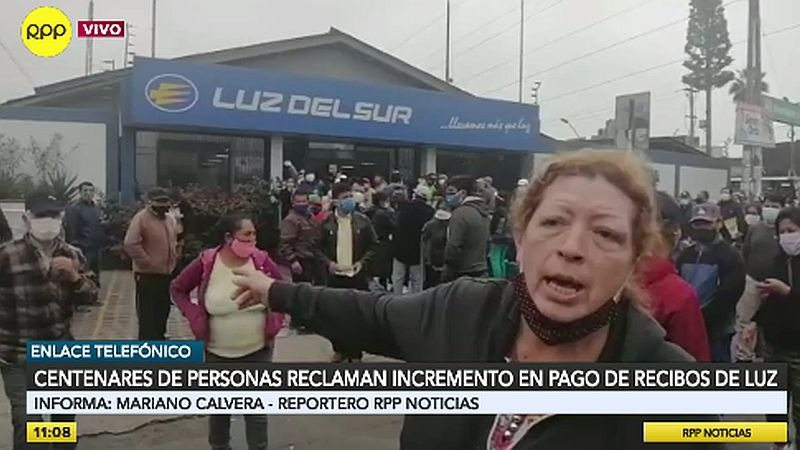
\includegraphics[width=0.65\textwidth]{motivacion}
\end{center}
\begin{center}
\vskip -0.5cm
\caption{\small{Noticias de la problemática en Lima - Perú}}
\label{fig:motivacion}
{\small{Fuente: \citep{WEBSITE:35}}}
\end{center}
\end{figure}

Entre el 16 de marzo y fines de junio de 2020, cuando el gobierno peruano declaró el estado de emergencia nacional por el COVID-19, las empresas generadoras de electricidad dejaron de enviar a su personal a las viviendas para realizar la lectura de los consumos en los medidores de energía eléctrica de los predios y facturaron por el consumo promedio de los seis meses anteriores. En muchos casos se encontró que los consumos normales habían crecido enormemente, en otros se duplicaron y hasta se triplicaron. Estas facturaciones generó miles de reclamos por cobros excesivos. %como se ilustra con la figura \ref{fig:noticia}.


\subsection{Antecedentes}
% y fundamentación científica, técnica o humanística}
En la actualidad existe una amplia variedad de sistemas relacionados a los BMS ofrecidos por empresas multinacionales tales como las que se describen a continuación:

\begin{itemize}

\item {Energy manager - Centraline}: solución de \emph{software} para gestión del consumo de energía.

%\vspace{0.25cm}
Es una nueva herramienta de \emph{software} de gestión energética profesional con el fin de lograr un ahorro importante y maximizar la eficiencia energética. El sistemas se ilustra con la figura \ref{fig:energy-vision} 

\begin{figure}[ht]
\begin{center}
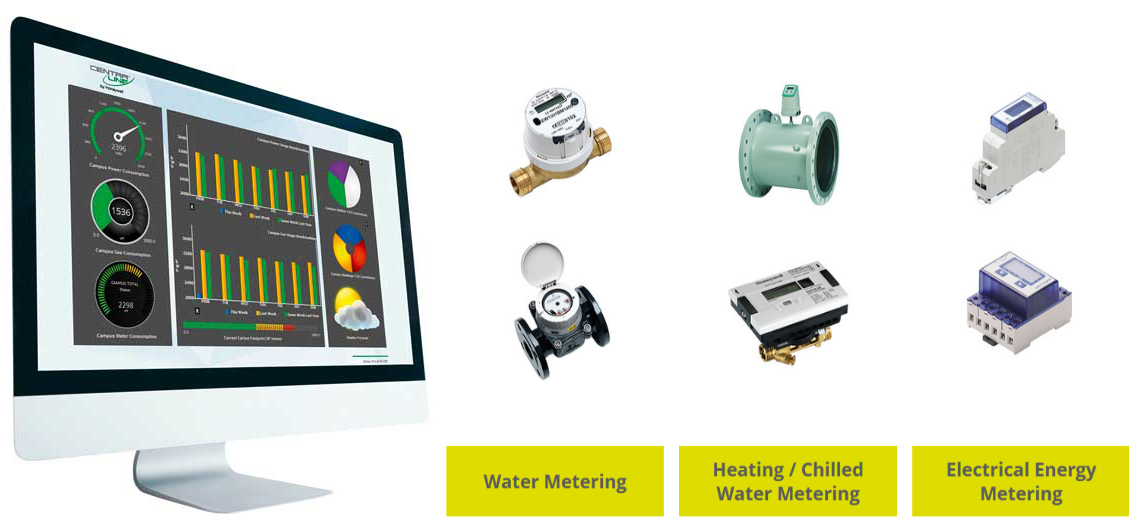
\includegraphics[width=0.7\textwidth]{energy-vision}
\end{center}
\begin{center}
\vskip -0.5cm
\caption{\small{Elementos del sistema Energy manager.}}
\label{fig:energy-vision}
{\small{Fuente: \citep{WEBSITE:13}}}
\end{center}
\end{figure}

%------------------------------
\item {Iammeter}: sistema de monitoreo de energía.

%\vspace{0.2cm}
Es un sistema de monitoreo de energía dedicado, al que se puede conectar medidores de energía Wi-Fi y luego comenzar a rastrear el uso de electricidad de su hogar o edificio comercial, y monitorear el flujo de energía del sistema fotovoltaico solar \citep{WEBSITE:11}.
%\vspace{0.15cm}
El sistema Iammeter puede generar un análisis integral del consumo de energía por usuarios, ofreciendo gráficos de datos y algunos detalles en el panel de información general. Ofrece el cálculo de la factura de la luz diaria/mensual y monitoreo en tiempo real del uso de electricidad \citep{WEBSITE:12}. El sistema se ilustra con la figura \ref{fig:iammeter}.

\begin{figure}[ht]
\begin{center}
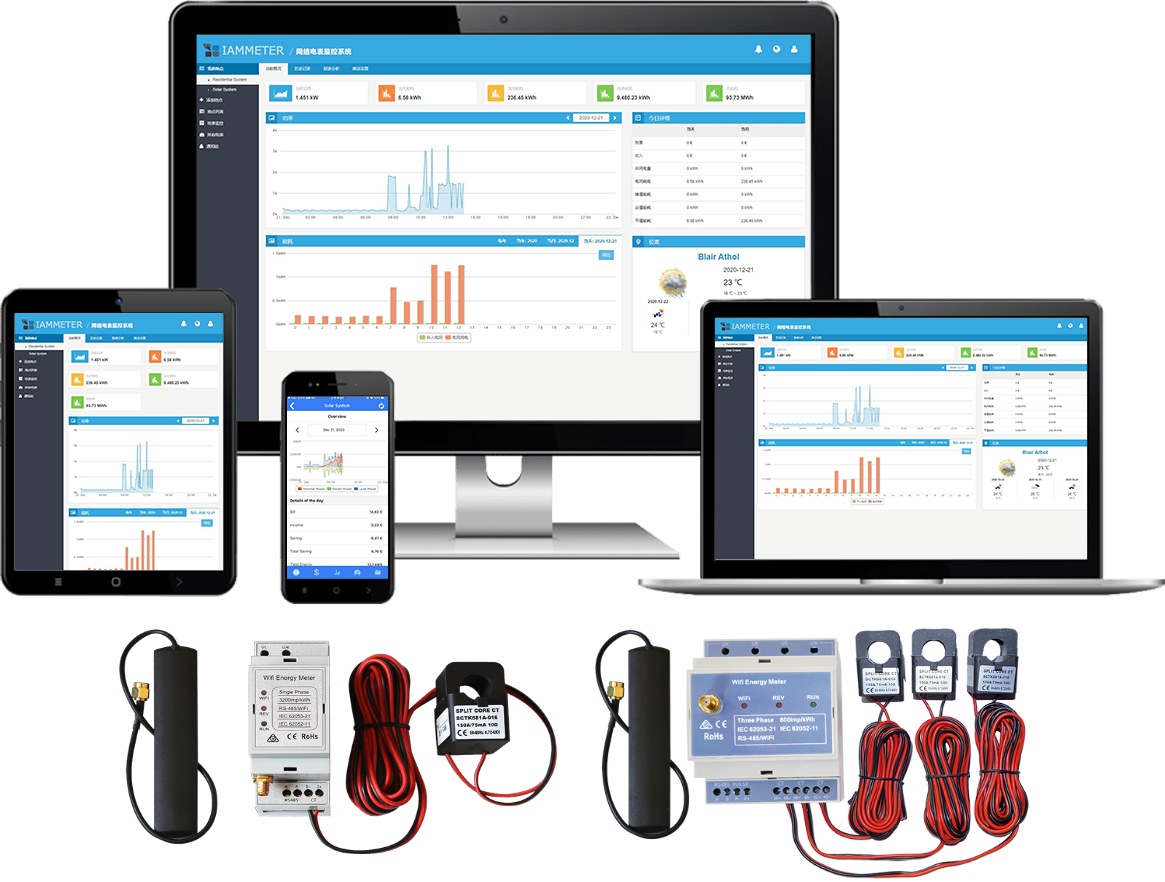
\includegraphics[width=0.65\textwidth]{iammeter}
\end{center}
\begin{center}
\vskip -0.5cm
\caption{\small{Elementos del sistema Iammeter.}}
\label{fig:iammeter}
{\small{Fuente: \citep{WEBSITE:11}}}
\end{center}
\end{figure}

Se puede acceder sistema desde todo tipo de dispositivos mediante un navegador con Internet o mediante su aplicación móvil.

%------------------------

\item {Bee2energy}: es una solución IoT basada en la nube a la que se puede acceder en cualquier momento y en cualquier lugar a través de Internet. Brinda operaciones en tiempo real con un modelo de negocio SaaS (\emph{\emph{software} as a service}) flexible y con capacidad multicanal \citep{WEBSITE:14}. Las funciones de control en edificios se ilustra con la figura \ref{fig:bee2energy2}.


\begin{figure}[ht]
\begin{center}
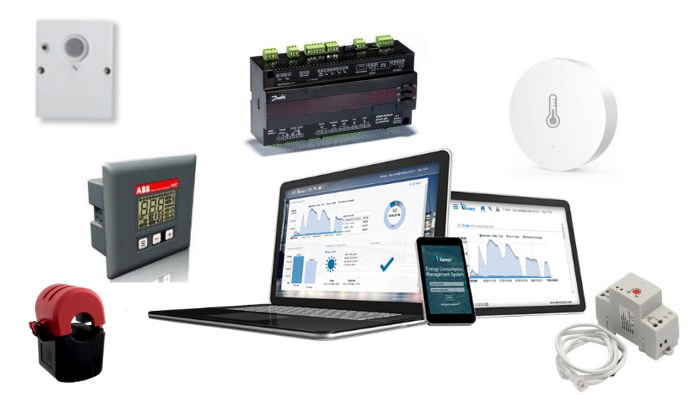
\includegraphics[width=0.7\textwidth]{bee2energy}
\end{center}
\begin{center}
\vskip -0.5cm
\caption{\small{Elementos del sistema Bee2energy.}}
\label{fig:bee2energy2}
{\small{Fuente: \citep{WEBSITE:14}}}
\end{center}
\end{figure}

Ofrece monitoreo en tiempo real de consumos, temperaturas, humedad y otros indicadores, configuración de reglas y encender / apagar equipos automáticamente o configurar alarmas y notificaciones.
\end{itemize}


%----------------------------------
Estos BMS fueron tenidos en cuenta para la toma de decisiones durante el desarrollo del proyecto, y por ello se resumen algunas de sus características en las tablas \ref{tab:tabla2} y \ref{tab:tabla3}:


%%%%%%%%%%%%%%%%%%%%%%%%%%%%%%%%%%%%%%
%escribir texto 2

\begin{table}[h]
	\centering
	\caption[Comparativa de soluciones entre acceso y servidor]{Comparativa acceso y tipo de servidor.}
	\begin{tabular}{l c c c c }    
		\toprule
		\textbf{Producto} & \textbf{Acceso} & \textbf{Servidor  local}   & \textbf{Servidor remoto} \\
		\midrule
		Energy Manager & local y remoto 	& no & sí  \\		
		Iammeter	 & local y remoto	& no & sí  \\
		Bee2energy	 & local y remoto	& no & sí  \\
		\bottomrule
		\hline
	\end{tabular}
	\label{tab:tabla2}
\end{table}

%\vspace{1cm}
%\vspace{1cm}

%%%%%%%%%%%%%%%%%%%%%%%%%%%%%%%%%%%

%escribir texto 3

\begin{table}[h]
	\centering
	\caption[Comparativa de soluciones entre protocolos y hardware]{Comparativa protocolos y tipos de hardware.}
	\begin{tabular}{l p{4.5cm} p{4cm} p{2cm}}    
		\toprule
		\textbf{Producto} 	 & \textbf{Protocolos}  & \textbf{ Sensores} & \textbf{Actuadores}  \\
		\midrule
		Energy manager & Modbus, M-Bus  y TCP/IP 	& propietario & propietario \\		
		Iammeter	 & MQTT y TCP/IP	& propietario /comercial & propietario\\
		Bee2energy	 & múltiples protocolos IoT		& propietario /comercial & propietario\\
		\bottomrule
		\hline
	\end{tabular}
	\label{tab:tabla3}
\end{table}








\subsection{Justificación}

Las necesidades de crear sistemas autómatas que permitan el control, seguridad, ahorro de energía y comunicación, son prestaciones que aportan valor añadido a la gestión técnica en los proyectos de edificaciones para los sectores público y privado creando entornos y ambientes que facilitan la habitabilidad y uso de una infraestructura moderna que aprovecha y hace uso de los diversos avances tecnológicos.

\vspace{0.25cm}
El desarrollo sostenible del país, ha permitido que en las últimas décadas los sectores productivos, tales como la industria, la construcción, la minería, entre otros, experimenten un auge y crecimiento de proyectos de inversión pública y privada. Para lo cual se genera la necesidad de contar con profesionales altamente capaces de aprovechar y desarrollar los diversos medios, elementos y avances tecnológicos en beneficio de la sociedad y los sectores productivos del país. \citep{ARTICLE:2}.

\vspace{0.25cm}
Por lo mencionado en los párrafos anteriores nuestra labor como profesionales con bases tecnológicas y científicas es crear los medios que permita acercar la tecnología a las personas, brindándoles un abanico de soluciones cada vez más amigables e informativas para que puedan conocer y usar. Por tanto, este proyecto busca ser una alternativa para aquellas personas que buscan una solución de automatización inteligente para sus viviendas u oficinas, así como brindarles la capacidad de interconexión de sus dispositivos por medio de nuestra plataforma.


\subsection{Problema}
¿De qué manera el desarrollo de un sistema BMS – IoT influye en el control automatizado del consumo eléctrico basado en el protocolo MQTT en viviendas multifamiliares, Trujillo 2023? 


\subsection{Hipótesis}
El desarrollo de un sistema BMS – IoT influirá significativamente en el control automatizado del consumo eléctrico basado en el protocolo MQTT en viviendas multifamiliares, Trujillo 2023.  


\subsection{Variables}

\vskip 0.2cm  
\subsubsection{Variables independientes}

\begin{itemize}
\item Intensidad de corriente.
\item Tensión eléctrica.
\end{itemize}

\subsubsection{Variables dependiente}
\begin{itemize}
\item Consumo eléctrico.
\end{itemize}

\subsection{Objetivos}

\vskip 0.2cm 
\subsubsection{Objetivo general}
\begin{itemize}
\item Desarrollar un sistema BMS - IoT para el control automatizado del consumo eléctrico basado en el protocolo MQTT en viviendas multifamiliares, Trujillo 2023.
\end{itemize}

\subsubsection{Objetivos específicos}
\begin{enumerate}
\item Diseñar una red IoT para un sistema BMS considerando las variables existentes en las viviendas multifamiliares.
\item Diseñar e Implementar la interfaz de comunicación y toma de datos de los sensores de forma simultanea mediante comunicación inalámbrica con el protocolo MQTT.
\item Diseñar e Implementar un módulo integrador - replicador de comunicación entre la red interna y la comunicación en la nube.
\item Diseñar e Implementar los módulos electrónicos con sensores y actuadores, para medir el consumo eléctrico doméstico.
\item Diseñar e implementar un software web responsivo a medida, para el sistema BMS - IoT.
\end{enumerate}



\subsection{Método de trabajo}
%De acuerdo con \cite{Erica}, para el desarrollo del método debe presentarse un bosquejo de la manera  en que se propone llevar a cabo la investigación, es decir, el camino a seguir o los pasos a seguir para realizar una cosa. Cuando mas complejo sea el bosquejo  más fácil se desarrollará el proceso de investigación. Se utiliza el vocablo método en vez de metodología, ya este último se considera equivocado, en el sentido en que se le utiliza comúnmente en informes de investigación. 
%\vskip 0.3cm
%Los tipos de métodos a usar para TG en informática, elegir un método, se considera:
%%%%%%%%%%%%%%%%\begin{enumerate}
%\item[a)] {\bf Método deductivo:} Es un método de razonamiento que consiste en tomar conclusiones generales para explicaciones partículares. El método se inicia con el análisis de los postulados, teoremas, leyes, principios, etc., de aplicación universal y de comprobada validez, para aplicarlos  a soluciones o hechos particulares. 

%\item[b)]{\bf Método cuantitativo:} Se fundamenta en la medición de las características de los fenómenos, lo cual supone derivar de un marco conceptual pertinente al problema analizado, una serie de postulados que expresen relaciones entre las variables estudiadas de forma deductiva, es decir, estudia fenómenos susceptibles de cuantificación y utiliza pruebas estadísticas para el análisis de datos. Este método tiende a generalizar y normalizar resultados. 

%\item[c)] {\bf Método inductivo:} Se utiliza el razonamiento para obtener conclusiones que parten de hechos particulares aceptados como válidos, para llegar a conclusiones, cuya aplicación sea de caracter general. El método se inicia con un estudio individual de los hechos y se formulan conclusiones universales que se postulan como leyes, principios o fundamentos de una teoría.

\textbf{Análisis y sintesis:} este método se eligió porque nos permite estudiar los hechos, partiendo de la descomposición del objeto de estudio en cada una de sus partes para estudiarlas en forma individual (análisis y estudio de sensores y actuadores), y luego se integran dichas partes para estudiarlas de manera holística e integral (síntesis del sistema IoT).
%%%%%%%%%%%%%%%%%%%%%%\end{enumerate}

\vskip 0.2cm 
Para lograr el objetivo se seguirá el flujo de trabajo ilustrado en la figura \ref{fig:diagrama} del gráfico del diagrama Activity On Node.

\begin{figure}[ht]
\begin{center}
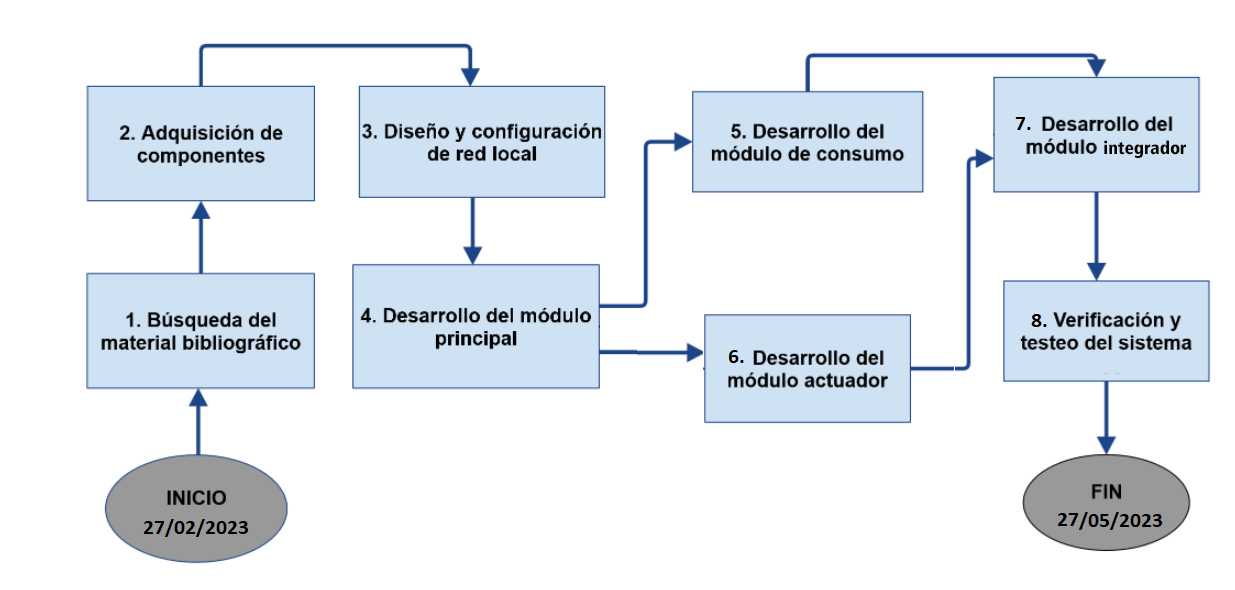
\includegraphics[width=0.82\textwidth]{AoN}
\end{center}
\begin{center}
\vskip -0.5cm
\caption{\small{Flujo del trabajo realizado.}}
\label{fig:diagrama}
\end{center}
\end{figure}


%Por lo tanto, plantear el objeto de estudio, el diseño de investigación a usar, las técnicas de recolección de la información a ser utilizadas, definir la población y tamaño de la muestra que debe ser representativa y necesaria para hacer generalizaciones, {\bf etapas del estudio} y análisis estadístico. El método de estudio entre otras cosas se refiere a la secuencia de pasos que se sigue para alcanzar los objetivos trazados, considerando los métodos propuestos anteriormente.\par
%\vskip 0.3cm
%{\bf Ejemplo:}\par
%\vskip 0.1cm
%Para llegar a los objetivos propuestos, el desarrollo de la investigación comprendió las siguientes etapas de trabajo a saber:
%\begin{enumerate}
%\item[a)] Análisis del problema de gestión de residuos sólidos urbanos (RSU) en el Brasil, para comprender la situación actual y levantar los principales cuellos de botella. Además, definir las principales variables de decisión para el modelamiento;
%\item[b)]	Levantamiento de los principales casos de éxito en la gestión de RSU en las ciudades brasileras, peruanas y de otros países;  
%\item[c)]	Formulación del problema principal de la investigación, justificando su importancia;
%\item[d)]	Levantamiento bibliográfico de los diferentes temas necesarios para la elaboración de la investigación, tales como Leyes de RSU, sustentabilidad, ruteo, logística urbana, logística reversa y gestión de residuos, entre otros;
%\item[e)]	Estudio y análisis de los modelos de ruteo, logística urbana y logística reversa que contribuyan con el estado de arte del problema formulado;
%\item[f)]	Estudio y análisis de los métodos de solución para resolver los modelos evaluados en la revisión bibliográfica, así como los modelos que serán propuestos en este estudio;
%\item[g)]	Investigación y estudio de software libre que permita el teste de los modelos estudiados y la implementación de los modelos desarrollados en la investigación;
%\item[h)]	Testes y validación de los modelos estudiados con la herramienta computacional escogida;
%\item[i)]	Planificación del sistema de logística reversa para la sustentabilidad en el contexto de la logística urbana, por medio del desarrollo del modelamiento matemático del Sistema de Colecta Selectiva (ruteo) y de Transporte de los RSU hacia los centros especializado para que sean reciclados, reutilizados o rechazados;
%\item[j)]	Elección de un área urbana para que sea utilizada como estudio de caso,  tanto para los testes de los modelos estudiados como de los modelos desarrollados;
%\item[k)]	Levantamiento de los datos necesarios para validar y testar los modelos junto a los organismos responsables y organizaciones que participan directa e indirectamente en este campo de trabajo;
%\item[l)]	Levantamiento de premisas y simulación de datos para ejecutar los programas, es decir, muchas veces las bases de datos reales que se encuentran son incompletas y por un determinado dato no se puede ejecutar el programa, en este caso, esas informaciones son llenadas por medio de simulaciones de datos considerando la experiencia del analista de sistemas;
%\item[m)]	Testes y validación de los modelos desarrollados en la ciudad escogida por medio de la generación de escenarios alternativos.    
%\end{enumerate}
    



%\subsection{Referencias}
%Presentar bibliografía conforme a las normas técnicas internacionales reconocidas: Un solo estilo American Psychological Association - APA. Seguir exactamente la forma de las referencias dadas como ejemplos. No usar numeros entre corchetes. Ver los ejemplos de las referencias dadas abajo.\par
\vskip 0.3cm
%Se exige como mínimo 10 referencias entre libros y/o artículos referentes al tema a investigar. Las referencias sustentan la investigación del TG.

\bibliography{Bibliografia} % Bibliografia formato APA


\vskip 1cm
\vskip 1cm
\vskip 1cm
\vskip 1cm
\vskip 1cm

\hspace{0.7cm}Daniel\hspace{.1cm}I.\hspace{.1cm} Cruz\hspace{.1cm}Flores 
\hspace{4cm}Leoncio\hspace{.1cm}M.\hspace{.1cm} Moya\hspace{.1cm}Carranza \\
\hspace*{2.6cm} Alumno  \hspace*{6.6cm}Alumno


\vskip 1cm
\begin{center}
Dra. \hspace{.1cm}Patricia\hspace{.1cm} Pereyra\hspace{.1cm}Salvador\\
 Asesor
\end{center}



\end{document}

